\documentclass{article}

\usepackage[slovene]{babel}
\usepackage[utf8x]{inputenc}
\usepackage{graphicx}
\usepackage[usenames,dvipsnames]{xcolor}
\usepackage[margin=5cm]{geometry}
\pagestyle{empty}

\begin{document}
\begin{center}
{\resizebox{11cm}{!}{\Huge\bf\color{OliveGreen} Angry Pigs}}\\[0.5cm]
{\huge \today}\ \\[2cm]
\end{center}
\section{Ekipa}
{\large Matic Potočnik (63060270)}\\
{\large Jaka Sivec (63070145)}
\section{Projekt}
Cilj projekta Angry Pigs je izdelati zabavno 3D igro, v kateri igralec s katapultom obstreljuje drevesa in skuša z njih sklatiti ptiče, ter njihova gnezda. V igri bo na voljo več različnih prašičev, položaj katapulta bo mogoče spreminjati, okolje pa bo v čim večji meri avtomatsko generirano, s poudarkom na drevesih.

Igra bo napisana ali v jeziku Clojure ali v jeziku Scala, z uporabo OpenGL knjižnice LWJGL.\\
\begin{center}
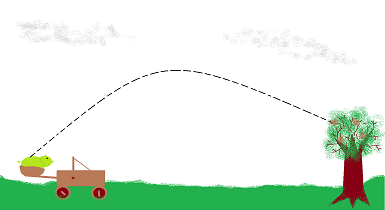
\includegraphics[width=6cm]{conceptsmall}
\end{center}

\end{document}